\begin{solution}
\begin{enumerate}
\item {[7 points]} Substituting the expressions for $u(x,y,t)$ and $f(x,y,t)$ into the partial differential equation yields
\[
\sum_{j=1}^\infty \sum_{k=1}^\infty a'_{j,k}(t) \psi_{j,k} (x,y)-\sum_{j=1}^\infty \sum_{k=1}^\infty a_{j,k}(t) \left(-\left(L\psi_{j,k}\right) (x,y)\right)=\sum_{j=1}^\infty \sum_{k=1}^\infty c_{j,k}(t) \psi_{j,k} (x,y)
\]
and hence
\[
\sum_{j=1}^\infty \sum_{k=1}^\infty \left(a'_{j,k}(t)+\lambda_{j,k}a_{j,k}(t)\right)\psi_{j,k} (x,y)=\sum_{j=1}^\infty \sum_{k=1}^\infty c_{j,k}(t) \psi_{j,k} (x,y).
\]
We can then say that
\begin{eqnarray*}
&&\sum_{j=1}^\infty \sum_{k=1}^\infty \left(a'_{j,k}(t)+\lambda_{j,k}a_{j,k}(t)\right)\int_0^1\int_0^1\psi_{j,k} (x,y)\psi_{m,n} (x,y)\,dx\,dy
\\
&=&\sum_{j=1}^\infty \sum_{k=1}^\infty c_{j,k}(t) \int_0^1\int_0^1\psi_{j,k} (x,y)\psi_{m,n} (x,y)\,dx\,dy,
\end{eqnarray*}
for $m,n=1,2,\ldots$, from which it follows that
\[
a_{m,n}'(t)+\lambda_{m,n} a_{m,n}(t)=c_{m,n}(t),
\]
for $m,n=1,2,\ldots$, since
\[
\int_0^1\int_0^1\psi_{j,k} (x,y)\psi_{m,n} (x,y)\,dx\,dy = \left\{\begin{array}{ll} 1 & \mbox{if }j=m\mbox{ and }k=n \\ 0 & \mbox{if }j\ne m\mbox{ or }k\ne n \end{array}\right.
\]
for $j,k,m,n=1,2,\ldots$.

Also,
\[
u(x,y,0)=0
\]
means that
\[
\sum_{j=1}^\infty \sum_{k=1}^\infty a_{j,k}(0) \psi_{j,k} (x,y)=0
\]
and so
\[
\sum_{j=1}^\infty \sum_{k=1}^\infty a_{j,k}(0) \int_0^1\int_0^1\psi_{j,k} (x,y)\psi_{m,n} (x,y)\,dx\,dy=\int_0^1\int_0^10\,dx\,dy,
\]
for $m,n=1,2,\ldots$, from which it follows that
\[
a_{m,n}(0)=0,
\]
for $m,n=1,2,\ldots$, since
\[
\int_0^1\int_0^1\psi_{j,k} (x,y)\psi_{m,n} (x,y)\,dx\,dy = \left\{\begin{array}{ll} 1 & \mbox{if }j=m\mbox{ and }k=n \\ 0 & \mbox{if }j\ne m\mbox{ or }k\ne n \end{array}\right.
\]
for $j,k,m,n=1,2,\ldots$, and
\[
\int_0^1\int_0^10\,dx\,dy=0.
\]

Hence, for $j,k=1,2,\ldots$, $a_{j,k}(t)$ is the solution to the differential equation
\[
a_{j,k}'(t)=-\lambda_{j,k} a_{j,k}(t)+c_{j,k}(t)
\]
with initial condition
\[
a_{j,k}(0)=0.
\]
\\
\item {[4 points]} For $j,k=1,2,\ldots$,
\begin{eqnarray*}
a_{j,k}(t) &=& \int_0^t e^{\lambda_{j,k}\left(s-t\right)} c_{j,k}(s)\,ds
\\
&=& \int_0^t e^{\lambda_{j,k}\left(s-t\right)} {(1+(-1)^j)(1+(-1)^k) (j^2\pi^2-24)\over 8 j^3 k \pi^4} e^{-s}\,ds
\\
&=& {(1+(-1)^j)(1+(-1)^k) (j^2\pi^2-24)\over 8 j^3 k \pi^4} \int_0^t e^{\left(\lambda_{j,k}-1\right)s-\lambda_{j,k}t}\,ds
\\
&=& {(1+(-1)^j)(1+(-1)^k) (j^2\pi^2-24)\over 8 j^3 k \pi^4} \left[{1 \over \lambda_{j,k}-1}e^{\left(\lambda_{j,k}-1\right)s-\lambda_{j,k}t}\right]_{s=0}^{s=t}
\\
&=& {(1+(-1)^j)(1+(-1)^k) (j^2\pi^2-24)\over 8 j^3 k \pi^4} \left({1 \over \lambda_{j,k}-1}e^{-t}-{1 \over \lambda_{j,k}-1}e^{-\lambda_{j,k}t}\right)
\\
&=& {(1+(-1)^j)(1+(-1)^k) (j^2\pi^2-24)\over 8 j^3 k \pi^4\left(\pi^2\left(j^2+k^2\right)-1\right)} \left(e^{-t}-e^{-\pi^2\left(j^2+k^2\right)t}\right).
\end{eqnarray*}
\\
\item {[4 points]} We can write
\begin{eqnarray*}
u(x,y,t) &=& \sum_{j=1}^\infty \sum_{k=1}^\infty a_{j,k}(t) \psi_{j,k}(x,y)
\\
&=& \sum_{j=1}^\infty \sum_{k=1}^\infty {(1+(-1)^j)(1+(-1)^k) (j^2\pi^2-24)\over 8 j^3 k \pi^4\left(\pi^2\left(j^2+k^2\right)-1\right)} \left(e^{-t}-e^{-\pi^2\left(j^2+k^2\right)t}\right) \psi_{j,k}(x,y)
\\
&=& \sum_{j=1}^\infty \sum_{k=1}^\infty {(1+(-1)^j)(1+(-1)^k) (j^2\pi^2-24)\over 4 j^3 k \pi^4\left(\pi^2\left(j^2+k^2\right)-1\right)} \left(e^{-t}-e^{-\pi^2\left(j^2+k^2\right)t}\right) \sin(j\pi x)\sin(k\pi y).
\end{eqnarray*}
\\
\item {[10 points]} Plots at the requested times are shown below, followed by the code that
generated them.

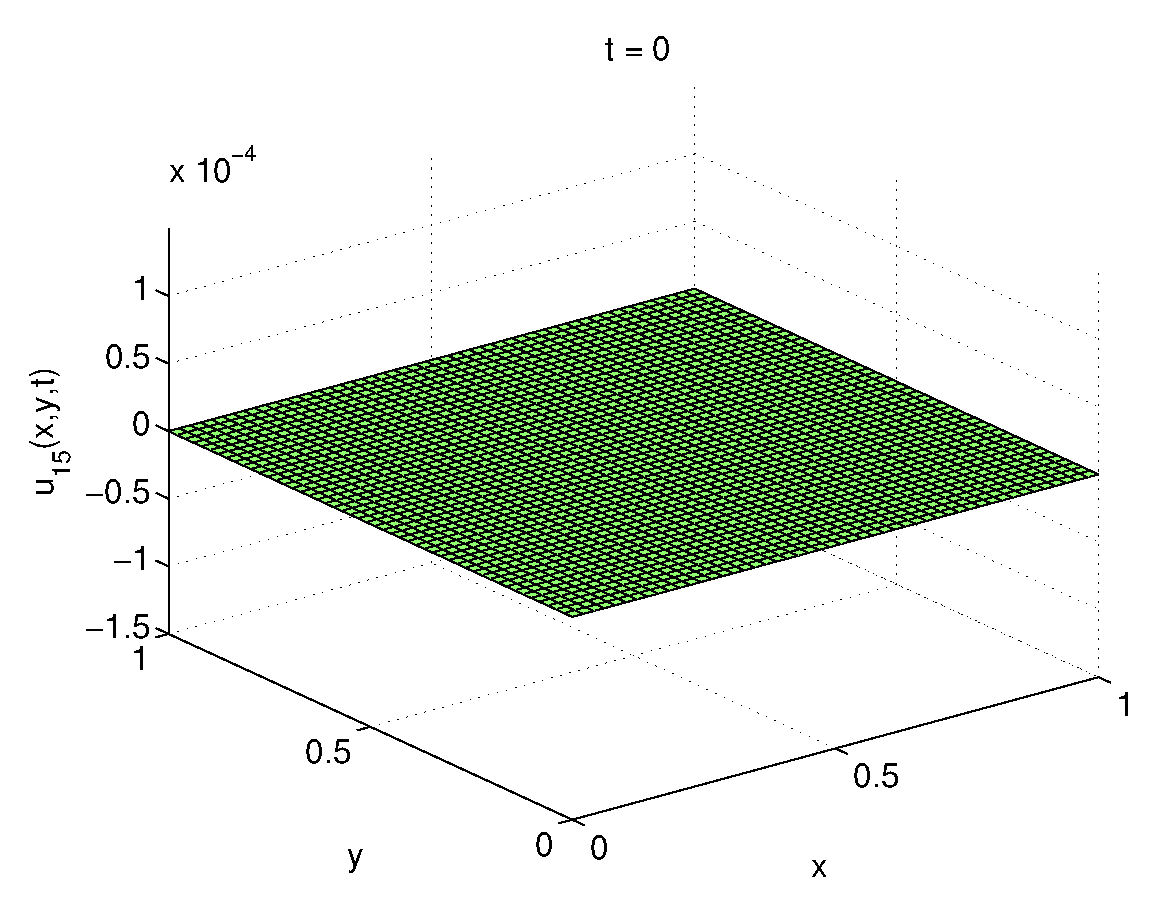
\includegraphics[scale=0.4]{heat2d1}
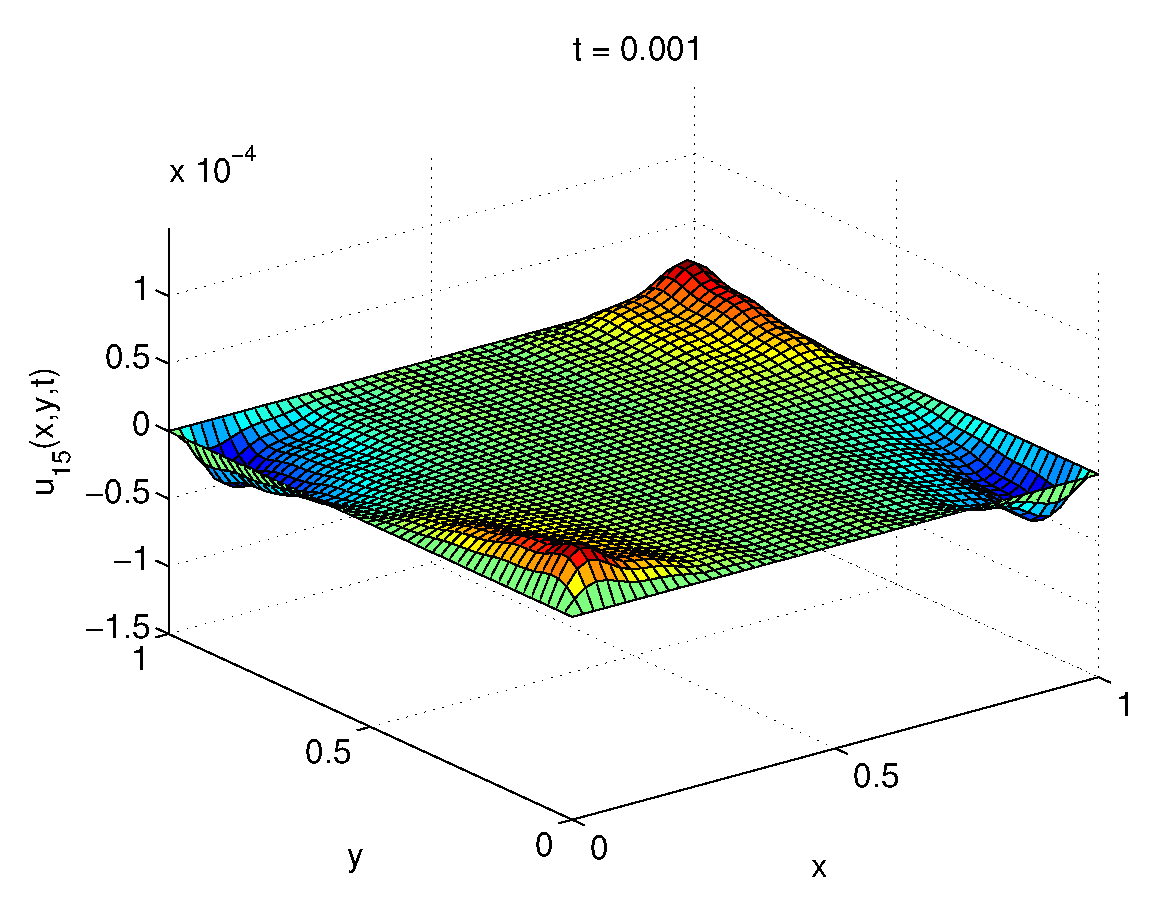
\includegraphics[scale=0.4]{heat2d2}

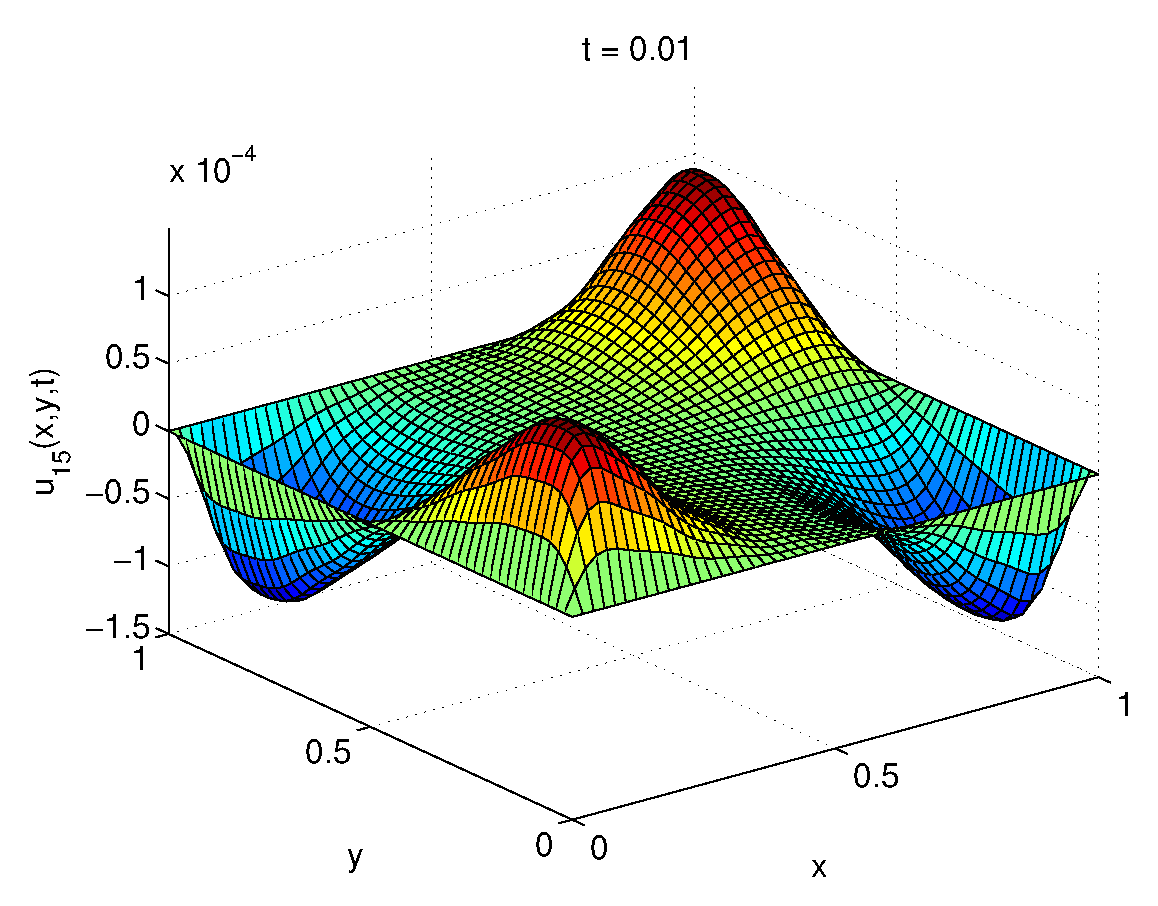
\includegraphics[scale=0.4]{heat2d3}
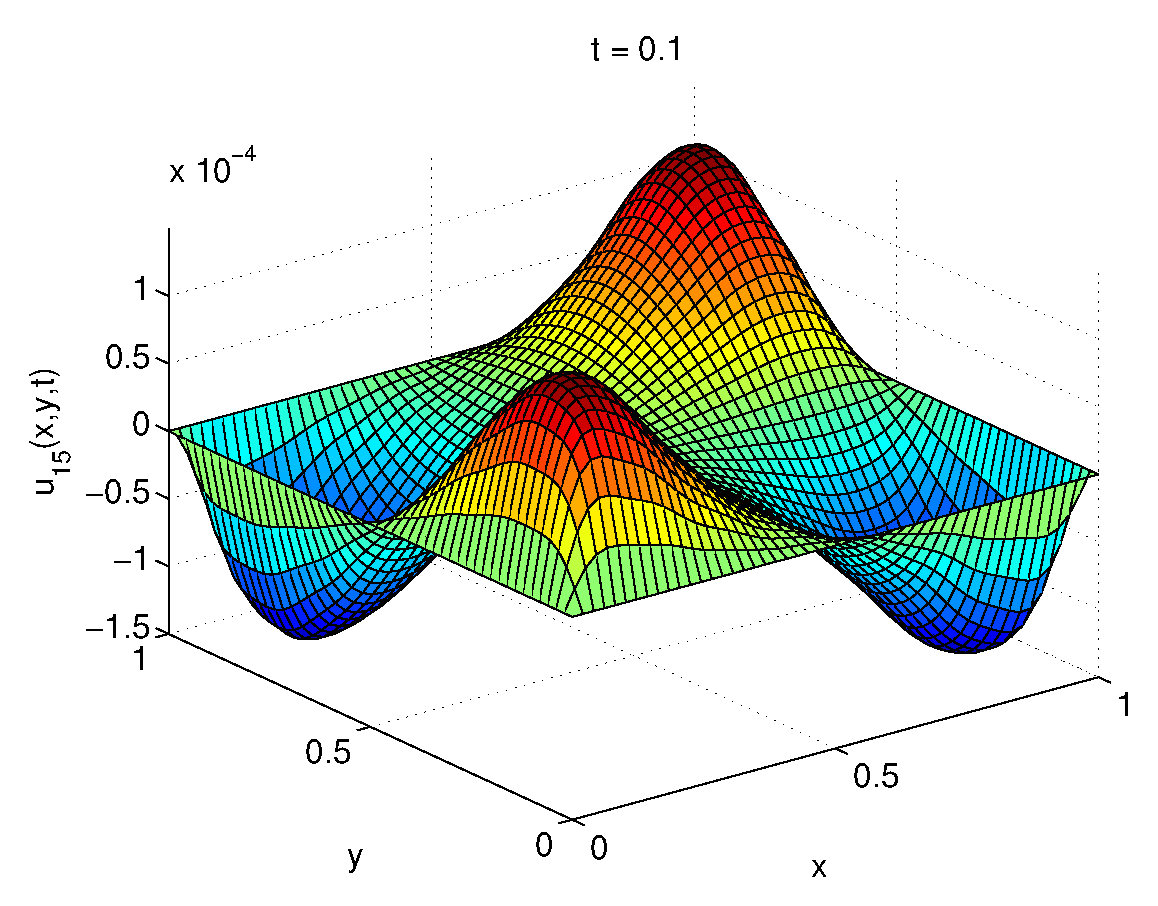
\includegraphics[scale=0.4]{heat2d4}

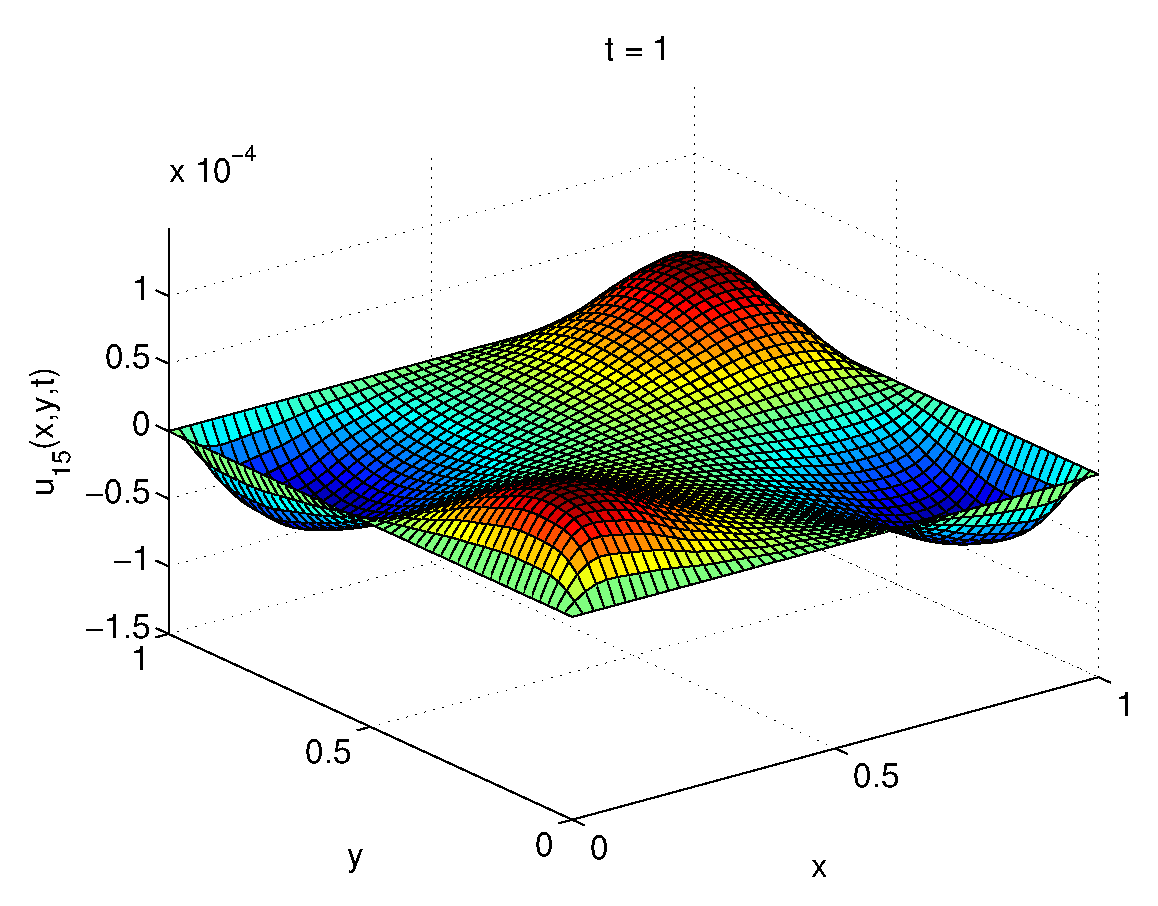
\includegraphics[scale=0.4]{heat2d5}
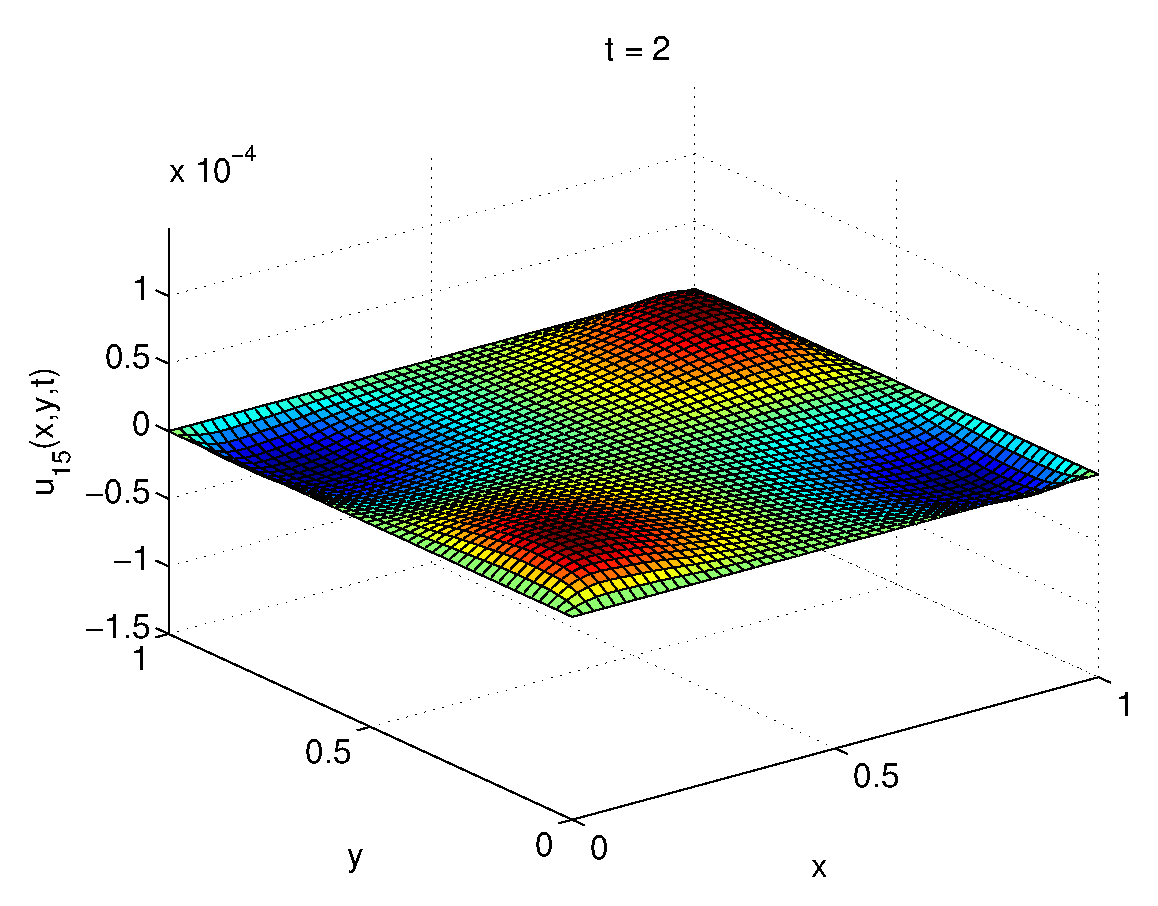
\includegraphics[scale=0.4]{heat2d6}

\lstinputlisting{HW43.m}
\end{enumerate}
\end{solution}